\section{Prosthesis Walking Control}\label{sec:back_walking_control}

\subsection{Time Based Control}
The earliest proposed robotic prosthesis control strategy, termed \emph{echo
control}, records the kinematics of the sound-side as a function of time leg on
each step and then executes an identical trajectory on the prosthesis side on
the following step \citep{grimes1977feasibility,grimes1979active}. Such a
control strategy has a number of drawbacks. First, the control strategy requires
measurement of the sound-side leg, thus burdening the amputee with additional
sensors that need to be donned and doffed daily. Second, the control is unable
to take an odd number of steps, and all steps must be initiated with the sound
leg. Third, the control is primarily, kinematic as measuring torques of the
sound side leg to use as a feedforward control on the prosthesis is infeasible.
Consequently, it may require high-gain feedback, which may cause discomfort and
gait instability due to a lack of compliance to the environment.  

Another form of time-based control, which we will use later in this thesis, is
the minimum jerk trajectory swing control presented in \citet{lenzi2014speed}.
This swing control strategy calculates at toeoff three minimum jerk
trajectories, parameterized by $5^\tn{th}$ order polynomials, which dictate the
movement of the knee and ankle joints. For the knee joint, two trajectories are
computed, one that starts at the position, velocity, and acceleration of the
knee at toeoff and goes to a peak flexion angle with zero velocity, and one that
starts at the peak flexion state and goes to a final state of zero angle,
velocity and acceleration. The peak knee angle is tuned to ensure adequate foot
clearance while the acceleration at the peak angle is based on able-bodied data.
For the ankle, one minimum jerk trajectory is used that starts at the position
and velocity at toeoff and proceeds to a final position, velocity, and
acceleration of zero. The durations of the trajectories are based on fixed
percentages of the stance duration thereby automatically adapting swing phase to
different gait speeds. Unlike the previously described echo control, this
control strategy takes advantage of the simple double-pendulum dynamics during
swing to derive a strong feedforward term that allows the use of small,
compliant feedback gains.

\subsection{Finite State Impedance Control}\label{sec:back_walk_fsm}
\begin{marginfigure}
    \centering
    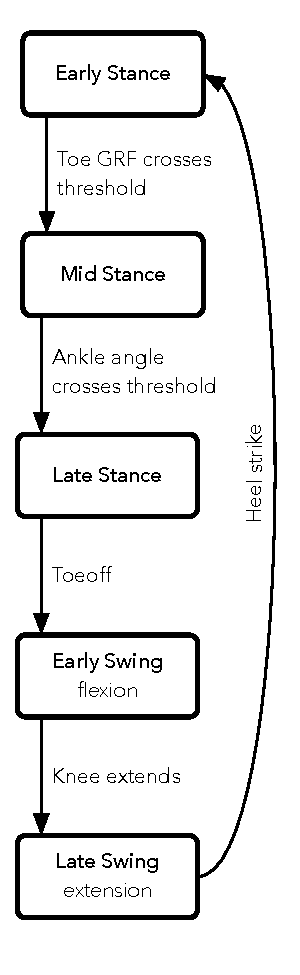
\includegraphics[width=\linewidth]{impedance_control_state_flow}
    \caption[Example finite state machine for the impedance control]{Finite
    state machine used for the impedance control scheme proposed in
    \citet{sup2009preliminary}. In each state the control employs linear
    impedance functions that determine the behavior of the ankle and knee joints
    of an active transfemoral
    prosthesis.}\label{fig:impedance_control_state_flow}
\end{marginfigure}
To alleviate issues with the time-based echo control, researchers later proposed
\emph{finite state impedance control}, which has become the most widely used
control for robotic legged prostheses. In this strategy, the gait cycle is split
into a sequence of discrete states or phases. During walking, a state machine
switches between the phases based on sensor data meeting certain conditions,
usually in the form of thresholds on joint angles, joint velocities, or ground
reaction forces. Within each phase, the controller specifies an impedance
relationship between the output torque at each joint and the angle and angular
velocity of that joint.

For example, \citet{sup2009preliminary}, proposes a specific instantiation of
this control paradigm in which the gait cycle is segmented into three stance
states and two swing states as shown in \cref{fig:impedance_control_state_flow}.
In each state, the impedance of a joint is governed by
\begin{align}
    \tau = -k (\theta - \theta_{0}) - b \dot \theta,\label{eq:impedance_func}
\end{align}
where $\tau$ is the desired torque of a joint, $k$ is a stiffness parameter
$\theta_{0}$ is the joint angle offset, $b$ is a damping parameter and $\dot
\theta$ is the joint velocity. If the stiffness, damping, and angle offset for
each joint and the transition rules are tuned appropriately, this control scheme
can be made to suit sloped walking \citep{sup2011upslope} and speed variations
\citep{shultz2016variable} including running \citep{shultz2015running}. There
have also been a number of variations on this general control scheme including
those with nonlinear impedance functions at the ankle
\citep{sup2007design,shultz2014walking} and some using high-gain position
control for the late stance push off phase of gait \citep{lawson2014robotic}.
\citet{lenzi2014speed} presents a similar strategy named \emph{quasi-stiffness
control} that substitutes the parameterized impedance functions given by
\cref{eq:impedance_func} with lookup tables that provide the torque vs angle
relationship at different gait speeds. 

A potential drawback of the impedance control paradigm may be its sensitivity to
the rules that govern transitions between phases. A premature transition or
delayed transition may cause inappropriate joint torques leading to gait
instabilities and falls. For this reason, prior works have experimented with a
wide variety of transition rules based on joint angles, velocities, and ground
reaction forces measured by the prosthesis. Alternatively, If one is willing to
instrument the sound-side leg, then \citet{liu2014improving} provides a method
to improve transition rules by using online learning and gait events of the
sound-side leg. In this thesis, however, we focus on control strategies that do
not require extra instrumentation of the body. Therefore, in later chapters we
will explore, through simulations (\cref{sec:control_sim}) and experiments with
our robotic prosthesis (\cref{sec:nm_vs_imp,sec:phase_estimation}), the
consequences of mistimed phase transitions in a finite state impedance control
scheme that does not use external sensing.

\subsection{Continuous Phase Control}\label{sec:back_walk_cont_phase}
Another approach to walking control in active prostheses is to estimate or
measure a continuous phase variable. This may avoid the gait instabilities that
can be caused by joint torques that change discontinuously in finite state
impedance control. Previous work in this area has focused on deriving phase
variables from single information sources. For example, \citet{gregg2014virtual}
enforce virtual constraints on the effective rollover shapes during walking.
The rollover shapes are the locations of the center of pressure (COP) in frames
attached to the shin and thigh. Proportional derivative control or feedback
linearization can be used to drive the error between the measured rollover shape
and desired rollover shape to zero. Typically, during walking the COP progresses
monotonically from heel to toe, making it an effective phase variable. However,
when walking on uneven terrain this assumption could be violated. Additionally,
this definition of phase is only applicable during stance.

To obtain a phase variable that is applicable in a wider variety of situations,
\citet{quintero2016preliminary} propose using the thigh angle and its integral
to derive a continuous phase variable. In this approach, one starts by plotting
in a chart the thigh angle on the $x$-axis and its (normalized) integral on the
$y$-axis. Assuming the thigh angle approximately follows a cosine trajectory
during gait, and with the right normalization and shift parameters, the thigh
angle/thigh angle integral form a circle over one gait cycle. Therefore, one can
use the polar angle of the thigh angle integral vs thigh angle as a phase
variable.  However, in order for the method to calculate a phase angle that
increases at a predictable constant rate, the thigh angle/integral plot should
be centered about the origin and the correct normalization needs to be applied
to the thigh integral.  Furthermore, in order for the thigh integral to reach
zero again at the end of a gait cycle, the average thigh angle must be
subtracted from the thigh angle before integration. The thigh angle shift,
integral shift, integral normalization, and angle average must be estimated
online in order to use this method. Incorrect estimation of these parameters can
cause the phase estimate to diverge. Consequently, using this method for
non-periodic motions is difficult.  In \cref{sec:back_walk_cont_phase} we
present our attempt to implement this style of control on our robotic
prosthesis. We found that the variability from step to step alone was enough to
cause significant drift in the thigh angle integral.  Thus we were not able to
achieve a consistent gait with this control scheme.

As a possible solution, \citet{rezazadeh2018phase} recently proposed a method
that eliminates the thigh angle integral and instead uses the thigh angle only.
This method relies on the insight that, for the most part, during gait the thigh
angle decreases monotonically from heel strike to shortly before toeoff, and
then increases from that point until the next heel strike. Therefore, one can
define two different relationships between the hip angle and phase for these two
portions of gait and use a finite state machine to transition between them.
However, reintroducing a finite state machine into the controller necessitates
tuning of transitions rules between phases and may cause similar issues as in
finite state impedance control.

Finally, \citet{azimi2019model} propose another approach to continuous
phase-based control of prostheses uses the forward translational hip position to
parameterize the desired gait trajectory. The trajectory is designed in
simulation subject to a partial hybrid zero dynamics constraint that allows one
to use a adaptive, control Lyapunov function-based, controllers with convergence
guarantees. However, to date, this control has only been used to actuate the
knee of a powered prosthesis while the ankle remained passive, perhaps due to
the additional complexity of dealing with multiple hybrid dynamics transitions
between swing, heel contact only, heel and toe contact, and toe contact only.

In \cref{sec:phase_estimation}, we propose an alternative approach to continuous
gait phase estimation that uses an extended Kalman filter to derive the phase
estimate. Unlike these reviewed approaches, the proposed approach can fuse
information from any combination of sensors that produce continuous output and
does not need a finite state machine. Moreover, we show the resulting control
can use the phase estimate to adapt to different gait speeds and enable
automatic transitions to standing mode. 

\subsection{Non Phase-Based Control}

So far, all walking controllers we reviewed keep track of either a discrete or
continuous estimate of phase during gait. However, researchers have also
proposed prosthesis controllers that do not take this approach. For example the
complementary limb motion estimation (CLME) approach proposed by
\citet{vallery2011complementary} uses linear regression to learn a direct
mappings between the angles and velocities of the user's limbs to the
prosthesis' joint angles and velocities. However, this approach used many IMUs
mounted to the torso and sound side leg to measure the user's kinematics, and
thus may be impractical for everyday use by an amputee.

Another class of non-phase based control uses neuromuscular models that simulate
the dynamics of the muscle tendon units in the leg and hypothesized reflex
pathways to generate the desired torques for walking. Prior work in simulation
of biped walking controlled by neuromuscular models has demonstrated that this
control approach can produce very natural and robust gait patterns
\citep{geyer2010muscle,song2013integration,song2015neural}.
\begin{marginfigure}[1in]
    \centering
    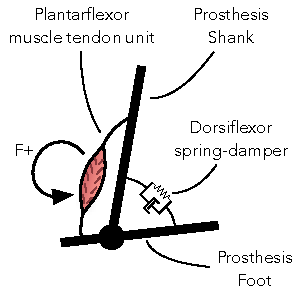
\includegraphics[width=\linewidth]{eilenberg_diagram} 
    \caption[Neuromuscular model used by \citet{eilenberg2010control} to control
    an active ankle prosthesis.]{Neuromuscular model used by
    \citet{eilenberg2010control} to control an active ankle prosthesis. During
    stance, a virtual muscle driven by positive force feedback, generates
    plantarflexion torque. During swing, a virtual spring and damper provides
    dorsiflexion torque to prevent toe scuffing.}\label{fig:eilenberg_diagram}
\end{marginfigure}
Motivated by the robustness and natural gait achievable by neuromuscular reflex
control, past research has applied this model to active ankle prostheses.
\citet{eilenberg2010control} applied a simplified version of the control to a
powered ankle prosthesis (\cref{fig:eilenberg_diagram}). In this work, the
neuromuscular model was reduced to a single ankle plantarflexor muscle driven by
a positive force feedback reflex during stance. During swing, the control
applies torque to dorsiflex the ankle according to a virtual spring-damper
model. In amputee testing of a prosthesis controlled by the neuromuscular model
the control produced ankle kinematics and kinetics similar to those observed in
healthy human walking. Significantly, \citeauthor{eilenberg2010control} found
evidence that the robustness  properties observed in neuromuscular model
simulations may carry over to amputee gait as well. The author's note that the
prosthesis automatically adapts torque output when walking on slopes, producing
more plantarflexion torque when walking up slopes and less when walking down
slopes. Additionally, \citet{markowitz2011speed} found that a similar
neuromuscular reflex model automatically produced more ankle plantarflexion work
as the amputee increased his gait speed.

The inclusion of user intent recognition via surface electromyography (EMG)
signals represents an interesting extension of neuromuscular reflex prosthesis
control. In these approaches, muscle activity in the residual limb is directly
measured via EMG sensors embedded in the amputee's prosthesis socket. These EMG
sensors are then used to control the torque generation of the amputee's leg
prosthesis. Because neuromuscular models describe how joint torque is generated
in response to muscle activations, a natural approach is to use the EMG signal
in reflex pathways in order to activate virtual muscles. This is the approach
proposed by \citet{wu2011electromyography}. In this work,
\citeauthor{wu2011electromyography} control an active transfemoral prosthesis
using EMG sensor readings from the residual thigh to activate virtual knee
flexor and extensor muscles according to a linearised Hill muscle model. The
resulting prosthesis control allowed an intact subject wearing the prosthesis
via an able-bodied emulator to achieve nearly normal gait. In a similar
approach, \citet{wang2013proportional} use EMG signals to modify the gain on a
positive torque feedback loop in order to control ankle plantarflexion torque.
As seen in healthy human walking, toe off angle and ankle net work increased
with increasing walking speed.
